\documentclass{article}
\usepackage{tikz}
% Packages for general formatting and mathematical symbols
\usepackage[utf8]{inputenc} % Encoding of your TeX file (UTF-8 is common)
\usepackage[T1]{fontenc} % Font encoding
\usepackage{amsmath, amssymb, amsthm} % Math packages
\usepackage{geometry} % Customizing page layout
\usepackage{parskip} % Adds spacing between paragraphs
\usepackage[ruled,vlined]{algorithm2e}
% Packages for graphics (optional)
\usepackage{graphicx} % For including images
\usepackage{float} % For precise placement of figures
\usepackage{appendix}
\usepackage{booktabs}
% Title and author information
\title{Resit Project 1}
\author{Jan van Ruijven 2006698}

\begin{document}

\maketitle % Display the title/author information

\section{Question 1}
First the data is split up into three parts: training, validation and testing. The training set is set te be 55\% of the data, the validation set 25\% and the testing set is 20\% of the data. 
The hyperparameters are split up into two catagories, the non-numeric hyperparameters which can be set to a specific value which is not a number. To this category belong the optimization algorithm, initialization and regularization. These hyperparameters are tested with the following values:
\begin{description}
	\item Optimization algorithm: Stochastic gradient descent and Adams optimizer
	\item Initialization: GlorotNormal and GlorotUniform
	\item Regularization: L1 and L2
\end{description}
\subsection*{Strategy}
The first step of the strategy is to first find the best combination of non-numerical hyperparameters. To test the non-numerical hyperparameters, a Neural Network is needed, to start things off the following Neural Network with numerical hyperparameters and one hidden layer is generated:
\begin{description}
	\item Number of nodes: 15  
	\item Batch size: 15
	\item Learning rate: 0.01
	\item Regularization rate: 0.01
\end{description}
After testing the non-numerical hyperparameters, the following combination seems to perform best on both the training and validation set: GlorotUniform initialization, Adams optimizer and L2 regularization.

The second step is to find the best combination of numerical hyperparameters. The idea is to increase and decrease the numerical hyperparameters and save the best performing combination, each time we do an iteration that is either not improving or seems te be overfitting on the data, the hyperparameters are being reset back to the best combination we have found so far. In each 10 fold of iterations we are changing the amount by which the hyperparameters are being adjusted, for the nodes and batch size, 10, 7, 4, 3, 2 and 1 are the sizes by which we are increasing and decreasing their values each 10 iterations respectively. For the regularization and learning rates the idea is completely similar, but now the amount is multiplied by 0.01. 

After running the strategy the following neural network is obtained:
\begin{description}
	\item Number of nodes: 7  
	\item Batch size: 21
	\item Learning rate: 0.006
	\item Regularization rate: 0
\end{description}
This Neural Network is able to produce a score of 0.11 on the testing set. A figure showing the best total score can be found in the appendix at figure \ref{fig:NN_learning}. In this figure it can be seen that the best performing network is found around iteration 50 and that the overal performance has large deviation in the beginning, but becomes more stable after around 30 iterations.

\newpage
\section{Question 2}
\subsection*{A}
\begin{equation}
	f(x) = 	W_{j1}^{2T} * a + b_1^2
	\label{eq:inside_step_function}
\end{equation}
In equation \ref{eq:inside_step_function} the function inside the stepfunction can be found. Here $a$ represents the output vector from the relu activation functions, this function can produce any non-negative output. Since the weights and biases can be controlled, any real number can be produced as long as the weights in equation \ref{eq:inside_step_function} can be set to both a positive and a negative value, which is the case. 
\subsection*{B}
To replicate the Relu activation function we need to apply the max function in linear fashion. This is done using a large number $M$, a binary variable $z$, a variable for adjustment $S$ and the output of the Relu function as $A$. To write everything out we first denote the following: the number of nodes is represented by $K$, the number of observations by $N$ and the number of parameters by $P$. To write out the Relu function the following is done:
\begin{align*}
    % Add ReLU constraints
    &A_{i, j} \leq (1 - Z_{i, j}) \cdot M \quad \text{for } i = 1, 2, \ldots, N, \quad j = 1, 2, \ldots, \text{K} \\
    &A_{i, j} \geq 0 \quad \text{for } i = 1, 2, \ldots, N, \quad j = 1, 2, \ldots, \text{K} \\
    \\
    &S_{i, j} \leq M \cdot Z_{i, j} \quad \text{for } i = 1, 2, \ldots, N, \quad j = 1, 2, \ldots, \text{K} \\
    &S_{i, j} \geq 0 \quad \text{for } i = 1, 2, \ldots, N, \quad j = 1, 2, \ldots, \text{K} \\
    \\
    % A's output equals the weights * input + bias for each node j and input i
    % here S is to make sure it's always a positive output (ReLU)
    &\sum_{p=1}^{P} W_{\text{eights1}, j, p} \cdot X_{\text{train}, i, p} + B1_j - A_{i, j} + S_{i, j} = 0 \\
    &\quad \text{for } j = 1, 2, \ldots, \text{K}, \quad i = 1, 2, \ldots, N
\end{align*}
Now that the first activation function is defined, the step function can be created, again the large number $M$ is needed to make sure that the output of the step function is less than 0 when our predicted value is 0 and the output is greater or equal than 0 when the predicted output value equals 1. To do this, the following constraints are created:
% if Y predict is 0, the sum of weights * activation plus bias is less than or equal to 0
\begin{align*}
    &\text{for } i = 1, 2, \ldots, N: \\
    &\quad \sum_{j=1}^{\text{K}} W_{\text{eights2}, j} \cdot A_{i, j} + B2 - Y_{\text{pred}, i} \cdot M \leq 0
\end{align*}
To produce the absolute value in the objective function, an auxilary variable must be created which is always greater or equal than the absolute value of the true value minus the predicted value.
% Add linearization constraints
\begin{align*}
    &\text{for } i = 1, 2, \ldots, N: \\
    &\quad Y_{\text{train}, i} - Y_{\text{pred}, i} \leq \text{aux}_i \\
    &\quad -Y_{\text{train}, i} + Y_{\text{pred}, i} \leq \text{aux}_i
\end{align*}
In an effort to stop the model from overfitting, L2 regularization is added. Therefore, the following objective value is obtained:
% Set objective function
\begin{align*}
    &\text{minimize } \sum_{i=1}^{N} \text{aux}_i + \lambda \left( \sum_{j=1}^{\text{K}} \sum_{p=1}^{P} W_{\text{eight1}, j, p}^2 \right. \\
    &\quad \left. + \sum_{j=1}^{\text{K}} B1_j^2 + B2 \right)
\end{align*}

\newpage
\section{Question 3}
After training and testing the neural network a training score of around 0.22 is found and a testing score of around 0.11. As for the MILP, when searching for the optimal solution, this is found relatively quickly and the predicted values equal the true values. But after testing the model either only 0's are returned, only ones, or random zeros and ones. I have tested a lot of different settings to try and reduce the overfitting, this would sometimes give very small improvements, but these seemed quite random. The improvements seemed random due to the fact that increasing my overfitting value lambda from 0.01 to 0.001001 would give a small improvement, but increasing it again by 0.000001 would have a negative effect. The overall advatage from the neural network over the MILP seems to be the fact that its easier to control for overfitting and underfitting while also producing good estimates. An MILP seems better in scenarios where (almost) identical data is inserted into the model each time, since the model can quickly find the optimal solution for one perticular set of input data.

\newpage
\appendix
\begin{figure}
	\begin{center}
/	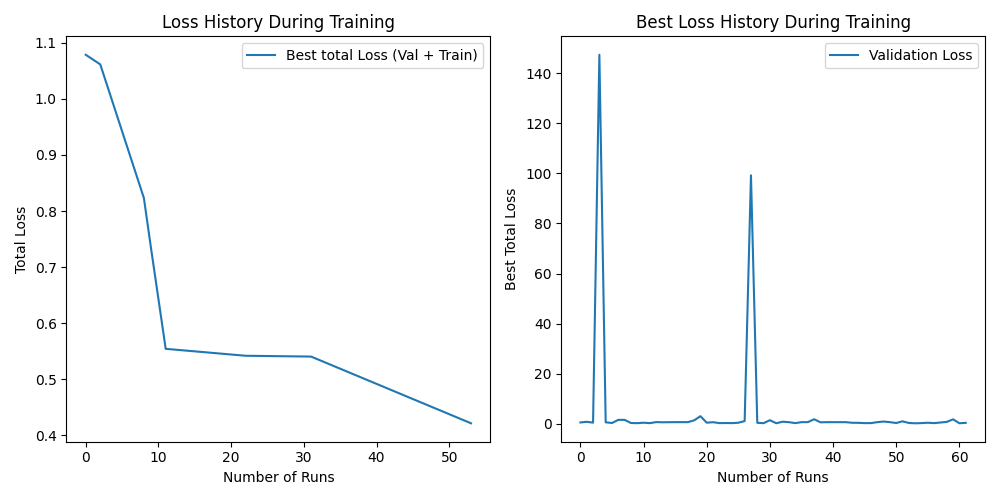
\includegraphics[width=0.95\textwidth]{figures/Figure_1}
	\end{center}
	\caption{Best total loss and overall validation loss over time}\label{fig:NN_learning}
\end{figure}


\end{document}
